% Figure 13: scale_lanes architecture at the CURRENT defaults (HARNESS_WHERE=session, SANDBOX_SESSIONS=0):
% 4 SGLang engines : 256 dispatchers : 256 fresh microVM sessions in flight. The agent loop runs INSIDE
% each session and dials its engine's adapter back over VPC; dispatchers only start + poll.
% Build: xelatex lanes_fig13_session.tex  (-> .pdf, included by ../agentcore_slime_deck.md)
\documentclass[tikz,border=4pt]{standalone}
\usepackage{fontspec}
\setmainfont{DejaVu Sans}
\setmonofont{DejaVu Sans Mono}
\usetikzlibrary{positioning,arrows.meta,fit,backgrounds,calc}
\definecolor{slime}{RGB}{230,230,230}
\definecolor{host}{RGB}{214,216,240}
\definecolor{gpu}{RGB}{255,236,204}
\definecolor{vm}{RGB}{214,238,220}
\definecolor{ink}{RGB}{40,40,90}
\begin{document}
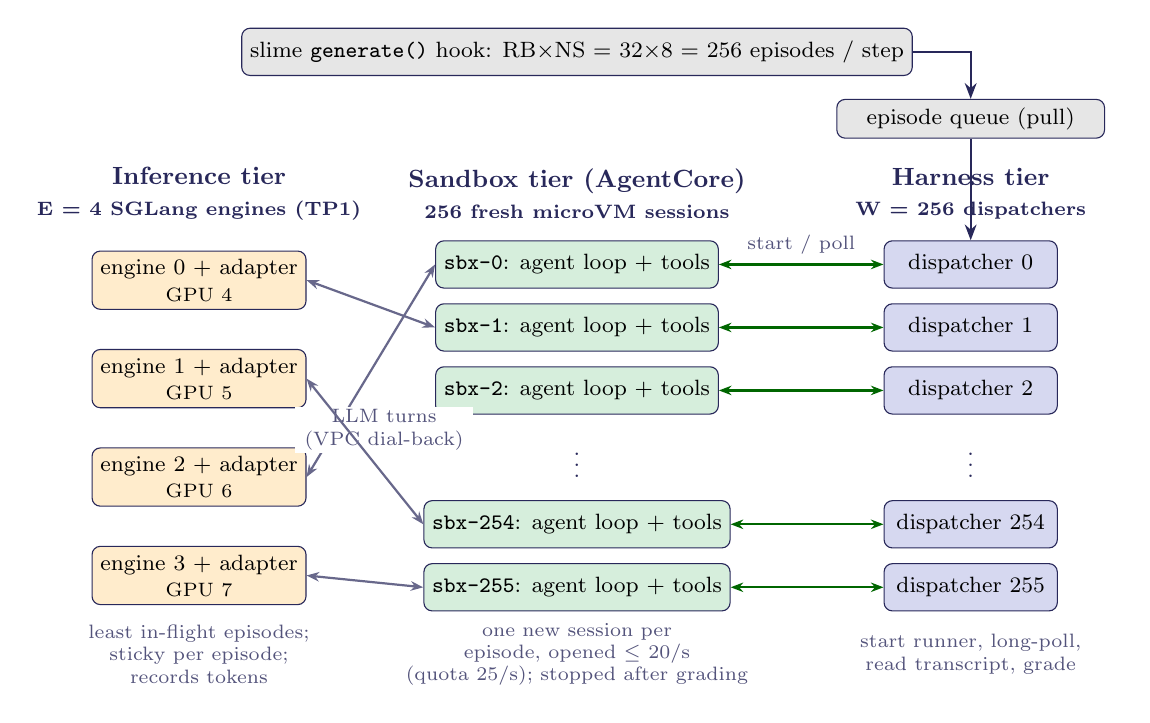
\begin{tikzpicture}[
  font=\footnotesize,
  box/.style={draw=ink, rounded corners=3pt, fill=#1, align=center, inner sep=3pt, minimum height=0.6cm, minimum width=2.2cm},
  line/.style={thick, draw=ink, -{Stealth[length=2mm]}},
  dline/.style={thick, draw=ink!70, {Stealth[length=1.6mm]}-{Stealth[length=1.6mm]}},
  head/.style={font=\small\bfseries, text=ink, align=center},
  note/.style={font=\scriptsize, text=ink!80, align=center, text width=3.6cm},
]

\node[box=slime, minimum width=5.4cm] (sl) at (5.2,2.7) {slime \texttt{generate()} hook: RB$\times$NS = 32$\times$8 = 256 episodes / step};
\node[box=slime, minimum width=3.4cm, minimum height=0.45cm] (q) at (10.2,1.85) {episode queue (pull)};
\draw[line] (sl.east) -| (q.north);

\node[head] at (0.4,0.9)  {Inference tier\\\scriptsize E = 4 SGLang engines (TP1)};
\node[head] at (5.2,0.9)  {Sandbox tier (AgentCore)\\\scriptsize 256 fresh microVM sessions};
\node[head] at (10.2,0.9) {Harness tier\\\scriptsize W = 256 dispatchers};

% engines (left)
\foreach \e/\y in {0/-0.2, 1/-1.45, 2/-2.7, 3/-3.95} {
  \node[box=gpu, minimum width=2.3cm] (e\e) at (0.4,\y) {engine \e\ + adapter\\\scriptsize GPU \the\numexpr\e+4\relax};
}
\node[note] at (0.4,-4.95) {least in-flight episodes;\\sticky per episode; records tokens};

% sessions (middle): agent loop + tools inside
\foreach \s/\n/\y in {0/0/0, 1/1/-0.8, 2/2/-1.6, 3/254/-3.3, 4/255/-4.1} {
  \node[box=vm, minimum width=3.1cm] (v\s) at (5.2,\y) {\texttt{sbx-\n}: agent loop + tools};
}
\node[text=ink] at (5.2,-2.45) {$\vdots$};
\node[note, text width=4.4cm] at (5.2,-4.95) {one new session per episode, opened $\le$ 20/s\\(quota 25/s); stopped after grading};

% dispatchers (right)
\foreach \w/\n/\y in {0/0/0, 1/1/-0.8, 2/2/-1.6, 3/254/-3.3, 4/255/-4.1} {
  \node[box=host] (h\w) at (10.2,\y) {dispatcher \n};
}
\node[text=ink] at (10.2,-2.45) {$\vdots$};
\draw[line] (q.south) -- (h0.north);
\node[note] at (10.2,-4.95) {start runner, long-poll,\\read transcript, grade};

% dispatcher -> session (start/poll)
\foreach \i in {0,1,2,3,4} { \draw[dline, draw=green!40!black] (h\i.west) -- (v\i.east); }
\node[note, above] at ($(h0.west)!0.5!(v0.east)$) {start / poll};

% session -> engine (LLM turns, VPC dial-back), crossing on purpose
\draw[dline] (v0.west) -- (e2.east);
\node[note, text width=2.2cm, fill=white, inner sep=1pt] at (2.75,-2.1) {LLM turns\\(VPC dial-back)};
\draw[dline] (v1.west) -- (e0.east);
\draw[dline] (v3.west) -- (e1.east);
\draw[dline] (v4.west) -- (e3.east);
\end{tikzpicture}
\end{document}
